%\documentclass[10pt,twocolumn,twoside]{IEEEtran}
\documentclass[journal]{IEEEtran}

% The following packages can be found on http:\\www.ctan.org
\usepackage{graphics} % for pdf, bitmapped graphics files
\usepackage{epsfig} % for postscript graphics files
\usepackage{mathptmx} % assumes new font selection scheme installed
\usepackage{times} % assumes new font selection scheme installed
\usepackage{amsmath} % assumes amsmath package installed
\usepackage{amssymb}  % assumes amsmath package installed
\usepackage{algorithm}
% \usepackage[utf8]{inputenc}
\usepackage[noend]{algpseudocode}
\usepackage{graphicx}
\usepackage[font=small,labelfont=bf]{caption}
\usepackage{epsfig}
\usepackage{ulem}
\usepackage{verbatim}
\usepackage{amsfonts}
\usepackage{mathrsfs}
\usepackage{breqn}
\usepackage{xcolor}
\usepackage{mathtools}
%\usepackage{varwidth}
%\usepackage{resizegather}
%\usepackage{euler}
\DeclarePairedDelimiter{\ceil}{\lceil}{\rceil}
\newcommand{\qd}{\hfill{\qed}}
\def\ba{\begin{array}}
\def\ea{\end{array}}
\newcommand{\beq}{\begin{equation}}
\newcommand{\eeq}{\end{equation}}
\newcommand{\bq}{\begin{eqnarray}}
\newcommand{\eq}{\end{eqnarray}}
\newcommand{\bqn}{\begin{eqnarray*}}
\newcommand{\eqn}{\end{eqnarray*}}
\newcommand{\bee}{\begin{enumerate}}
\newcommand{\eee}{\end{enumerate}}
\newtheorem{definition}{Definition}


\RequirePackage{ifthen}
\usepackage{amssymb,mathrsfs,wasysym}
\usepackage{tikz}
\usepackage{url}
\usetikzlibrary{shadows}
\usetikzlibrary{shapes}

\newcommand{\always}{\square}
\newcommand{\eventually}{\Diamond}
\renewcommand{\next}{\ocircle}
\newcommand{\until}{\hspace{1mm}\mathcal{U}\hspace{1mm}}
\newcommand{\untilc}{\mathcal{U}}
\newcommand{\release}{\hspace{1mm}\mathcal{R}\hspace{1mm}}
\newcommand{\true}{\relax\ifmmode \mathit{True} \else \em True \/\fi}
\newcommand{\false}{\relax\ifmmode \mathit{False} \else \em False \/\fi}
\newcommand{\aand}{\hspace{1mm}\wedge\hspace{1mm}}
\newcommand{\oor}{\hspace{1mm}\vee\hspace{1mm}}
\newcommand{\set}[1]{\left\{#1\right\}}
\newcommand{\norm}[1]{\left\lVert#1\right\rVert}

% correct bad hyphenation here
% \hyphenation{op-tical net-works semi-conduc-tor}

\setlength{\textfloatsep}{10pt plus 1.0pt minus 2.0pt}
\begin{document}

\title{Receding Horizon Synthesis and Dynamic Allocation of UAVs to Fight Fires}

\author{Joshua~Shaffer,~
	Estefany~Carrillo,~
	and~Huan~Xu, Member, IEEE\vspace*{-7mm}% <-this % stops a space
\thanks{E. Carrillo is with the Department of Electrical and Computer Engineering, 
	University of Maryland, College Park,
  	MD 20740, USA e-mail: ecarril2@terpmail.umd.edu.}
\thanks{J. Shaffer and H. Xu are with the Department of Aerospace Engineering,
	University of Maryland, College Park,
	MD 20740, USA e-mail: \{jshaffe9, mumu\} @umd.edu.}
\thanks{This work was partially funded by Lockheed Martin.}}% <-this % stops a space


% As a general rule, do not put math, special symbols or citations
% in the abstract or keywords.

\maketitle



% As a general rule, do not put math, special symbols or citations
% in the abstract or keywords.
\begin{abstract}
This paper explores the design of a high-level mission planner and controller for managing UAVs fighting a wildfire through the utilization of reactive synthesis and dynamic allocation of the UAVs as resources to the fires. Reactive synthesis provides a formal means of guaranteeing the UAVs transition to areas of fire, refill on water, and emergency land as defined by LTL specifications. Dynamic allocation coordinates the behavior of multiple UAVs through assignments to regions of fire based on a cost function that takes into effect the fire locations, fire intensities and other UAV locations. For six fire scenarios, this paper determines the minimum number of UAVs required to eliminate all fires and prevent the burning of more than a set amount of fuel (i.e. forestry or shrubbery). Lastly, our results and successful application expand discussion on the utilization of reactive synthesis in larger task spaces and the implications of abstracting UAV transitions for use in formal methods.
\end{abstract}

% Note that keywords are not normally used for peerreview papers.
%\begin{IEEEkeywords}
%Controller synthesis, Allocation processes, Receding Horizon control, Linear Temporal Logic.
%\end{IEEEkeywords}


% For peer review papers, you can put extra information on the cover
% page as needed:
% \ifCLASSOPTIONpeerreview
% \begin{center} \bfseries EDICS Category: 3-BBND \end{center}
% \fi
%
% For peerreview papers, this IEEEtran command inserts a page break and
% creates the second title. It will be ignored for other modes.
\IEEEpeerreviewmaketitle
\vspace*{-4mm}
\section{Introduction}
% The very first letter is a 2 line initial drop letter followed
% by the rest of the first word in caps.
% 
% form to use if the first word consists of a single letter:
% \IEEEPARstart{A}{demo} file is ....
% 
% form to use if you need the single drop letter followed by
% normal text (unknown if ever used by the IEEE):
% \IEEEPARstart{A}{}demo file is ....
% 
% Some journals put the first two words in caps:
% \IEEEPARstart{T}{his demo} file is ....
% 
% Here we have the typical use of a "T" for an initial drop letter
% and "HIS" in caps to complete the first word.

\IEEEPARstart{T}{he} economic burden of wildfires on the United States (in 2016 \$US) exceeds \$63.5 billion annually due to damages, and more than \$7.6 billion is spent annually to fight said fires \cite{c0}. Current methods of fighting fires involve numerous man hours and piloted vehicles capable of dropping large amounts of suppressant over regions of fire. As discussed in \cite{c1}, unmanned aerial vehicles (UAVs) pose a huge benefit to traditional firefighting methods by providing additional ``eyes in the sky" and supply drops, which has motivated numerous agencies to explore such options in the last decade. Furthermore, UAVs could potentially extinguish fires on their own as was mechanically demonstrated on a small, single-UAV scale in \cite{c2}. Fighting wildfires primarily through a fleet of autonomous drones, in turn, could limit the number of required personale and produce more efficient results. For the purposes of research in UAV autonomy, a design problem such as this allows for the exploration and further assessment of multiple methods in automation.

One such method, reactive synthesis, provides a means for generating correct-by-construction controllers for complex systems. Synthesized controllers take into account system and environment variables with varying dynamics, progress and safety specifications, and initial conditions. The primary benefit of this method is the correct-by-construction attribute: the realized controller will satisfy the specifications designed by the user as long as the environment behaves according to the assumptions made. Programmers are not required to ``handcraft" individual behaviors of a system under specific conditions (of which are often error prone) and can instead focus on defining the system and specifications. The major pitfall of reactive synthesis is the computational complexity in dealing with dynamic environments as discussed in \cite{c10}.

Despite such disadvantages, the implementation of reactive synthesis is suitable when considering finite abstractions of systems with small state spaces. Without this type of framework, most problems become infeasible to handle only with reactive synthesis. For example, consider a scenario involving the path planning of a robot that must always avoid any number of arbitrarily placed obstacles on a 10x10 grid. The synthesized controller must account for every possible obstacle location ($2^{100}$ permutations), resulting in an inordinate amount of computation time. Unfortunately, real problems can easily involve this scenario's scale of permutations in the environment, hence the restrictions enforced on reactive synthesis. 

When the high-level design of a system does involve this scale of environmental permutations and state space, solutions typically seek to discretize the synthesis problem or approach the problem from a different perspective. Discretization appears in the use of receding horizon control in \cite{c3} and the use of decentralized controllers for multiple agents in \cite{c4}. Both examples break down the top-level synthesis problem into smaller, discrete pieces for the computation benefits. On the other hand, \cite{c5} approached their synthesis problem with a focus on resolving deadlock under specific environment conditions instead of directly avoiding dynamic obstacles. In each of the presented cases, the problem description focuses on a limited task space and how the solution can handle larger sets of actions from an environment. In \cite{c3}, \cite{c4}, and \cite{c5}, the task space encompasses up to 4 progress statements for each scenario. 
%Even with the problem space discretized, both examples presented rely on other methods to achieve the desired results. In [CITE],... and in [CITE]... Clearly a gap still exists between designing the high-level controllers for robust autonomous systems that reside within reality and utilizing reactive synthesis to fully realize such designs. In truth, attempting to close the gap presents a futile challenge, one that .... 

For the purposes of fighting large, dynamic fires with a single autonomous UAV, a high-level controller created with just reactive synthesis would quickly present an impractical solution if the design should accommodate a fairly granular state space with a large number of tasks. Further expanding this concept to a whole fleet of UAVs, the problem becomes worse due to an increase in the number of system variables. Even with decentralized controllers for each UAV, more system variables would need to be introduced to describe coordination and behaviors between the decentralized UAV controllers. To alleviate the computational complexity on reactive synthesis in this regard, the coordination of UAVs can be handled by a dynamic allocation process. %As discussed, the more arbitrary the scenario is (preferred given the idea that a single design should fit for most applications), the more likely that a design based solely on reactive synthesis would become impractical due to increased permutations in environmental variables. \textcolor{red}{REVISE SOME}%As discussed later on in this paper (in the \textit{Implementation} section), breaking down the synthesis problem still provided excessive state spaces to explore, and the futility of attempting a singular synthesized solution became readily apparent.

Dynamic allocation presents an autonomous method for assigning resources in an ever-changing environment. Recent approaches include clustering techniques and formulating the allocation problem in the form of a multi-objective problem. In \cite{c14}, a partitioning-based task allocation strategy is proposed to decide on the assignment of agents in dynamic disaster environments by applying the K-means clustering algorithm. In \cite{c15} and \cite{16}, the resource allocation problem is framed as a multi-objective optimization problem of minimizing the extinguishing time and resource utilization cost, solved by the use of evolutionary algorithms in \cite{c15} and by mathematical programming techniques in \cite{16}. 

We propose an allocation strategy to address the assignments of UAVs for our fire fighting scenario. If the fleet of UAVs are treated as resources to manage with respect to a changing fire landscape, dynamic allocation would serve well in assigning the UAVs to specific fires. Assignments would depend upon factors in the behavior of the fires such as density, intensity, ability to spread, and more. Perhaps readily apparent, though, is that an allocation algorithm would not necessarily be constructed to control the UAVs within the state space defined, nor would the algorithm manage other high-level system aspects associated with the UAVs, such as suppressant control and decisions on emergency landings. Building these high-level behaviors into an allocation algorithm requires ``handcrafting" these behaviors for all scenarios, an approach that synthesis, on the other hand, is well suited to avoid.

To integrate the two discussed methods, reactive synthesis and dynamic allocation, we utilize the receding horizon framework for reactive synthesis as discussed in \cite{c10}. As far as we have found, \cite{c6} first touched upon the idea of manipulating the receding horizon framework for decomposing the synthesized problem and decentralizing the planning procedure. For their purposes, this idea resulted in the ability of multiple agents to satisfy high-level specifications through only considering other agents that entered their local horizon. For our purposes, decentralizing the planning procedure allows for dynamic allocation to arrange the order of progress goals specified in the synthesized controller in real-time. Through this, we seek to reconcile the strengths and weaknesses of the two discussed methods to create a high-level mission planner and controller for implementation in a fire fighting scenario. 

%This paper is motivated by the concept of combining reactive synthesis with other methods to work in tandem and provide a solution to a high-level problem with a large number of tasks to achieve. We seek to build upon the work described above by exploring a multi-agent system in a complex dynamic environment while meeting a task-space on an order of magnitude greater than the aforementioned task spaces. 

The rest of the paper follows as such. In \textit{Section II}, we present subjects pertinent to the exploration of our topic, primarily in relation to reactive synthesis. In \textit{Section III}, we present the fire fighting scenario, including environment and system definitions. \textit{Section IV} discusses our proposed solution, followed by the implementation of our solution in \textit{Section V}. In \textit{Section VI}, we present the outcomes to our tested cases, followed by our conclusions in \textit{Section VII}.

\vspace*{-3.5mm}
\section{Preliminaries}

\subsection{Linear Temporal Logic}
To begin, linear temporal logic (LTL) is utilized for describing specifications within the reactive synthesis framework. Given a set $S$ of variables with a finite domain to describe a system (or environment), $s$ represents a state of said system (or environment). An atomic proposition (AP) $p$ is a statement on the system variables, evaluating either true or false. If the given state elements at any moment result in true for an atomic proposition, we show $s \models p$, otherwise we show $s \not\models p$.

LTL itself is built through APs with logic connections and temporal modal operators. Logic connections include $\lnot$ (negation), $\lor$ (or), $\land$ (and),  and $\longrightarrow$ (implication). Temporal modal operators include $\next$ (next), $\always$ (always), $\eventually$ (eventually), and $\until$ (until). An AP is an LTL formula formed through the finite variable set $S$, and propositional formulas (denoted with $\varphi$) are special cases of APs consisting of only logic connections. LTL formulas are interpreted over an infinite sequence of the states used to describe them, such as $\sigma = s_1 s_2 s_3 ... s_i ... s_{\infty}$. For any LTL formula $\varphi$, we state that $\varphi$ holds at position $i \geq 0$ of $\sigma$ if $s_n \models p$ for $n \geq i$. Through the use of APs constructed around system states, a broad range of specifications can be written to describe the behaviors of any system (or environment). We point the reader to the preliminaries section of \cite{c7} for an expanded description of LTL as it pertains to our purposes.

\vspace*{-3.5mm}
\subsection{Reactive Synthesis}
Reactive synthesis provides a method for generating controllers within the context of a defined environment and system. Specifications written in LTL are utilized to describe the desired behavior of the system and environment. One of the most commonly used forms for these LTL formulas is general reactivity(1) (GR(1)), the assume-guarantee form shown in (\ref{GR1}),
\begin{equation}
\label{GR1}
\begin{aligned}
(\varphi_{init}^{e} \land \bigwedge_{i \in I_r} \always \varphi_{s,i}^{e} \land \bigwedge_{i \in I_f} \always \eventually \varphi_{p,i}^{e}) \longrightarrow \\ (\varphi_{init}^{s} \land \bigwedge_{i \in I_s} \always \varphi_{s,i}^{s} \land \bigwedge_{i \in I_g} \always \eventually \varphi_{p,i}^{s}).
\end{aligned}
\end{equation}
From the above equation, the propositional formula $\varphi_{init}$  describes the initial condition of the environment or system (denoted by superscript $e$ or $s$, respectively), $\varphi_{s,i}$  describes safety specifications, and $\varphi_{p,i}$ describes progress specifications. Safety specifications describe properties that should always be fulfilled, while progress statements describe properties that should always eventually be fulfilled. \cite{c7} proved that when the system and environment specifications are written in the framework shown in (\ref{GR1}), the synthesis of a system controller that fulfills the system specifications while subject to the environment specifications will occur in polynomial time $N^3$. The proof of such, though, provides no guarantee that the polynomial time required will fall within a practical time-limit, due to the formulation's limiting dependency on the total amount of permutations between the system and environmental states.

\vspace*{-3.5mm}
\subsection{Receding Horizon}

\begin{figure}
	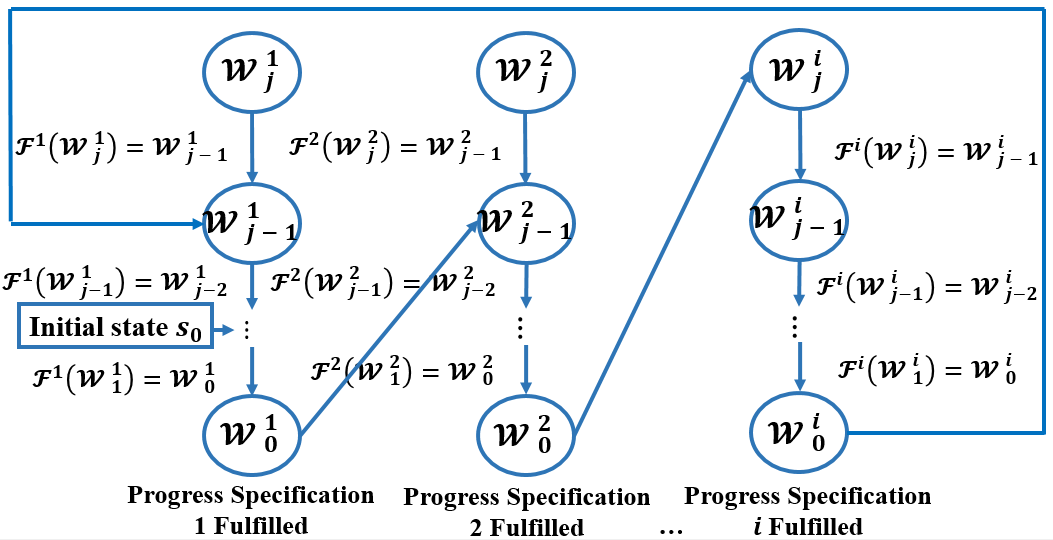
\includegraphics[width = 1 \linewidth]{RHFramework}
	\centering
	\caption{Segmentation of state space and example of ordered set flow-down performed in receding horizon framework, as described in \cite{c10}.}
	\label{RhFrame}
	\vspace*{-3mm}
\end{figure}

\cite{c8}, \cite{c9}, and \cite{c10} have explored reactive synthesis within a receding horizon (RH) framework. The primary benefit of utilizing RH is the segmentation of the state space for both the environment and system into separate horizons. Each horizon provides a smaller problem to synthesize a controller for, and the combination of these controllers form a single controller that obeys the specifications written for the total system and environment. The primary disadvantage of RH is that while each horizon itself can be optimized, the total sum is not. Other sources have explored methods of optimizing control with respect to time-based rewards on each horizon, such as in \cite{c9}, but any time-based optimization is forgone in this paper. 

Implementation of RH revolves around, for each progress specification, segmenting the total system state space into regions $\mathcal{W}_j^i$ so that, when placed into properly constructed ordered sets represented by $\mathcal{F}^i(\mathcal{W}_j^i)$, the system variables will converge to meeting each progress statement for the system, i.e. $\mathcal{W}_0^i$. Here, $i$ represents the system progress statement $i \in I_g$, and $j$ indexes the ordered regions $\mathscr{W}$ about the progress specification $i$. This process is displayed in Fig. \ref{RhFrame}. Following the basis laid out by \cite{c10}, each region consists of its own GR(1) specification (shown in (\ref{RH})), constructed so that the synthesized controller will move the system states towards the next region within the ordered set (eventually leading to $j = 0$) and fulfill the top level GR(1) specification,

\begin{equation}
\label{RH}
\begin{aligned}
\Psi_{j}^{i} = ((s \in \mathcal{W}_j^i) \land \Phi \land \bigwedge_{i \in I_r} \always \varphi_{s,i}^{e} \land \bigwedge_{i \in I_f} \always \eventually \varphi_{p,i}^{e}) \longrightarrow \\
(\bigwedge_{i \in I_s} \always \varphi_{s,i}^{s} \land \always \eventually(s \in \mathcal{F}^i(\mathcal{W}_j^i)) \land \always \Phi).
\end{aligned}
\end{equation}

In (\ref{RH}), $s$ refers to the system state. The formula $\Phi$ consists of all limitations on the states of system, preventing the system from making transitions to or initializing within states that are not allowed. This tautology prevents individual synthesized controllers from creating transitions to states that are infeasible for longer horizons.

\vspace*{-4mm}
\section{Problem Formulation}
The high-level problem scenario this paper explores is presented as such. A region of forest and/or grassland, segmented by various large-scale obstacles, is experiencing a wildfire. The fire spreads from starting points with a fixed behavior, and the starting fire conditions are arbitrary, i.e. any number of fires can occupy any number of subdivisions in the region that contain fuel to burn. A base of operations exists near the edge of the region and contains a fleet of $N$ UAVs for fighting the fire. Each UAV holds a varying level of water for dumping on the fire, from High (100\%), Medium (60\%), Low (20\%), to Empty (0\%), associated with a total water volume of $W_v = $ 50 liters. Each individual UAV contains a radio for communicating with base, GPS for determining position, and any other sensors required for lower-level controllers. Each UAV's average flight speed, $v$, is approximately $15$ m/s.

 \begin{figure}
	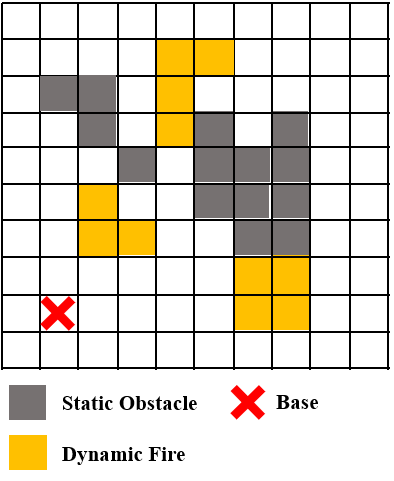
\includegraphics[width = 0.6 \linewidth]{GridPartitionVert}
	\centering
	\caption{2D grid partition of problem location with environmental indicators}
	\label{probpartition}
	\vspace*{-3mm}
\end{figure}

 \begin{figure}
	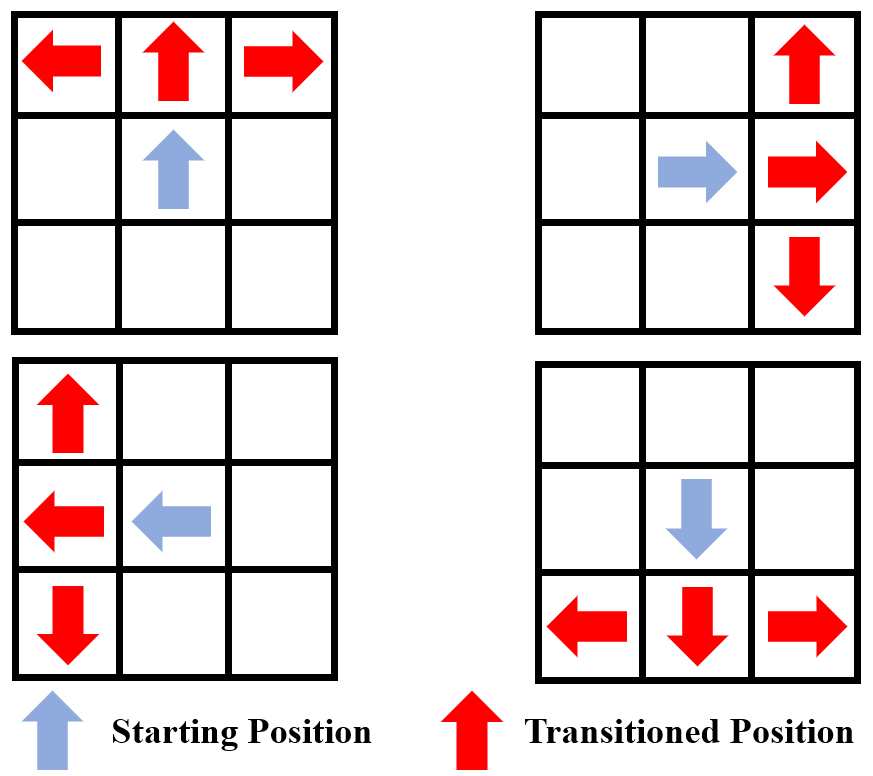
\includegraphics[width = 0.6 \linewidth]{Transitions}
	\centering
	\caption{Possible transitions for UAV within grid given starting orientation and location}
	\label{transitions}
	\vspace*{-3mm}
\end{figure}

For the purposes of this paper, suppose that the overall 2D region is partitioned into a granular 10x10 grid, as shown in Fig. \ref{probpartition}, with each partition side measuring at $l = 45$ meters. Each partition that is not an edge of the region or does not hold an obstacle is capable of experiencing fire within it. UAVs can transition throughout these partitions in the manner displayed in Fig. \ref{transitions} and have the ability to stop within a partition, indicating emergency landing. Every transition represents $l/v = 3$ seconds in real-time. From the above descriptions, the set of states of the UAVs, $S$, consist of their position in the grid, $s_{p}$, and orientation, $s_o \in \{1,2,3,4\}$. Additionally, the UAVs' states include the water level, $w \in \{0,1,2,3,4\}$ (each level tied to the percentages described before), and therefore $S = s_p \times s_o \times w$.

 \begin{figure}
	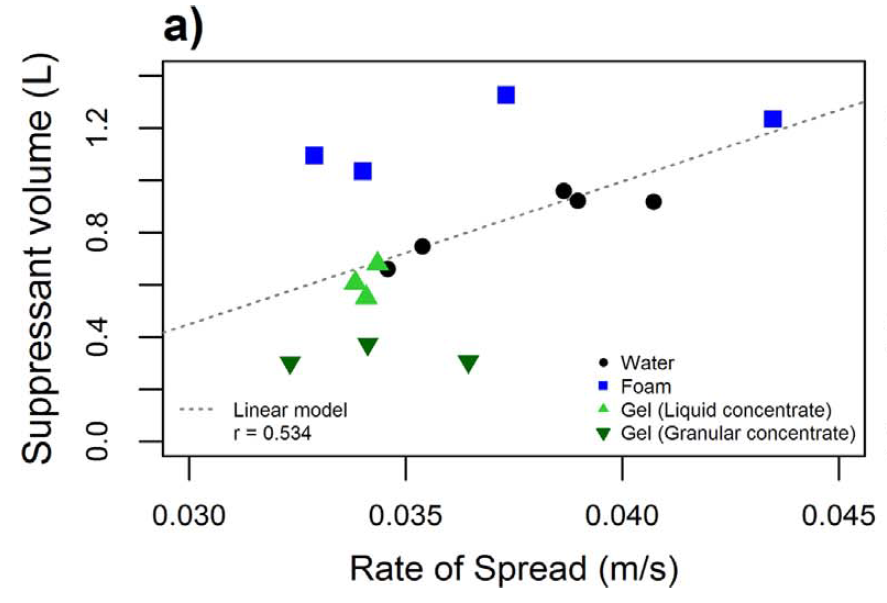
\includegraphics[width = 1.0 \linewidth]{FireRateCITE}
	\centering
	\caption{Tested suppressant volumes required for extinguishing fires per spread rates in 1.5 x 3 meter test area, pulled directly from \cite{c11}}
	\label{FireRateSpread}
	\vspace*{-3mm}
\end{figure}

The fire behaves as described. Each partition can contain $f \in \{0,1,2,3,4,5,6\}$ amount of fuel (i.e. forestry or shrubbery), starting with $f = 6$ for all partitions capable of holding fire. This results in an initial total fuel amount of $F = 300$ (subtracting region edges and obstacles). The fuel amount corresponds to how long a fire can burn within a partition, and as long as it is greater than $0$, the partition can hold a fire. Each fire varies in intensity, with levels of Low, Medium, and High, that are each tied to a specific fire spread rate, $f_r$. These rates, shown in Table \ref{table_1}, were pulled from the results data gathered in \cite{c11} and shown in Fig. \ref{FireRateSpread}. From the same test data, each rate requires a specific volume of water per square meter, $v_r$, to extinguish. A fire will grow in intensity and spread to adjacent partitions with time, $t_f$, determined by the partition length, $l$, divided by the spread rate of the fire. Each time a fire grows in intensity, all adjacent partitions that do not currently hold fire and do contain fuel will start holding fire, matching the intensity of the originating fire. Additionally, the fire will consume fuel in the partition, an amount described by $f_c$, proportional to its intensity level. Each of above described properties are listed in Table \ref{table_1}.

\begin{table*}[t]
	\centering
	\caption{Fire growth behavior}
	\label{table_1}
	\scalebox{1}{
		\begin{tabular}{|c||c||c||c||c|}
			\hline
			\multicolumn{1}{|p{3cm}|}{\centering Fire intensity level} & \multicolumn{1}{|p{3cm}|}{\centering Fire spread rate $f_r$ (m/s)} & \multicolumn{1}{|p{3cm}|}{\centering Required suppressant volume per square meter $v_r$ (L/m\textsuperscript{2})} & \multicolumn{1}{|p{3cm}|}{\centering Time before fire spreads $t_f$ (s)} & \multicolumn{1}{|p{3cm}|}{\centering Fuel consumption at intensity increase $f_c$} \\ 
			\hline
			Low & 0.035 & 0.156 & 1287 & 1 \\ 
			\hline
			Medium & 0.040 & 0.211 & 1125 & 2 \\
			\hline
			High & 0.045 & 0.267 & 999 & 3 \\
			\hline
		\end{tabular}
	}
\vspace*{-3mm}
\end{table*}

Each time one or multiple UAVs drop a combined amount of water, labeled $v_{ud}$, on a partition with fire, the total volume of water dropped on that partition, $V_d$, grows by $v_{ud}$. Furthermore, if $V_d$ reaches the necessary amount $v_r$ (provided in Table \ref{table_1}) for the given fire intensity \textit{before} the fire grows and spreads, the partition is considered extinguished with the current fuel amount, and fire can no longer spread to that partition. If the fire spreads before this volume of dropped water is reached, then $V_d$ resets to $0$. %These rules are detailed further in the \textit{Implementation} section.

%\textcolor{red}{()}. This equation, while not determined directly by a physical law, is created to capture an effectiveness of coordination in UAVs, a desired behavior of the UAVs detailed later on. The equation shows that each time a combined amount of water is dropped, the amount registered as effective to the fire scales around a nominal amount of 40\% of the total tank amount $W_v$.

%\begin{equation}
%\begin{aligned}
%V_d = V_d + v_{ud}*(W_v*(1 - 0.40) + v_{ud})
%\end{aligned}
%end{equation}

Desired design specifications for each individual UAV are as follows. Each UAV must only drop a fraction of its water supply (transitioning from the currently held amount to next lowest) when flying over designated fire regions, and each UAV must return to base for replenishing water supplies when $w = 0$. Additionally, the UAVs may experience engine problems and must land for prolonged periods of time in the next available region not consumed by fire. Lastly, the UAVs must coordinate when asked, either prioritizing the same fires with multiple UAVs or different fires for each UAV. 

As mentioned before, the design goal for this problem scenario is to create a high-level autonomous controller to dictate the overall behavior of the fleet for tackling any generic fire situation while maintaining the desired design specifications per UAV. For a given fire scenario, we seek to determine the required minimum number of UAVs. Given any number of UAVs, success is achieved when the fleet can permanently extinguish all fires while maintaining a minimum level of total fuel.

\vspace*{-3mm}
\section{Proposed Solution Method}
We propose a solution method to the formulated problem scenario that combines reactive synthesis with a dynamic allocation algorithm. These two methods form a high-level planner and controller that fulfills the design constraints imposed on each UAV and dictates the behavior of each one as well as their collective maneuvers. Fig. \ref{RHAlloc} depicts a conceptual view of the process of creating our solution and the duties that each method fulfills. Fig. \ref{AllocandGoal} depicts the direct relationship between the allocation process and a synthesized controller.

\begin{figure}
	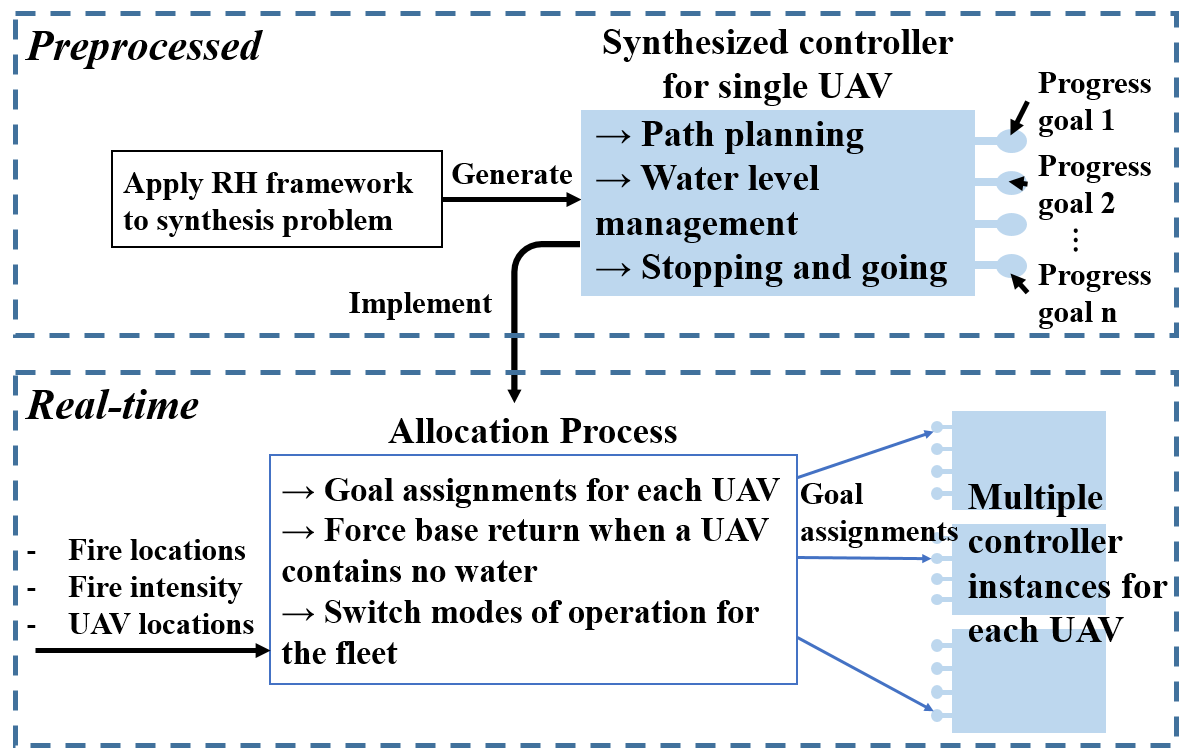
\includegraphics[width = 1.0 \linewidth]{SynthAlloc}
	\centering
	\caption{Diagram of creating the solution method and the responsibilities and roles for both the synthesized controllers and the allocation process during real-time implementation}
	\label{RHAlloc}
	\vspace*{-3mm}
\end{figure}

 \begin{figure}
	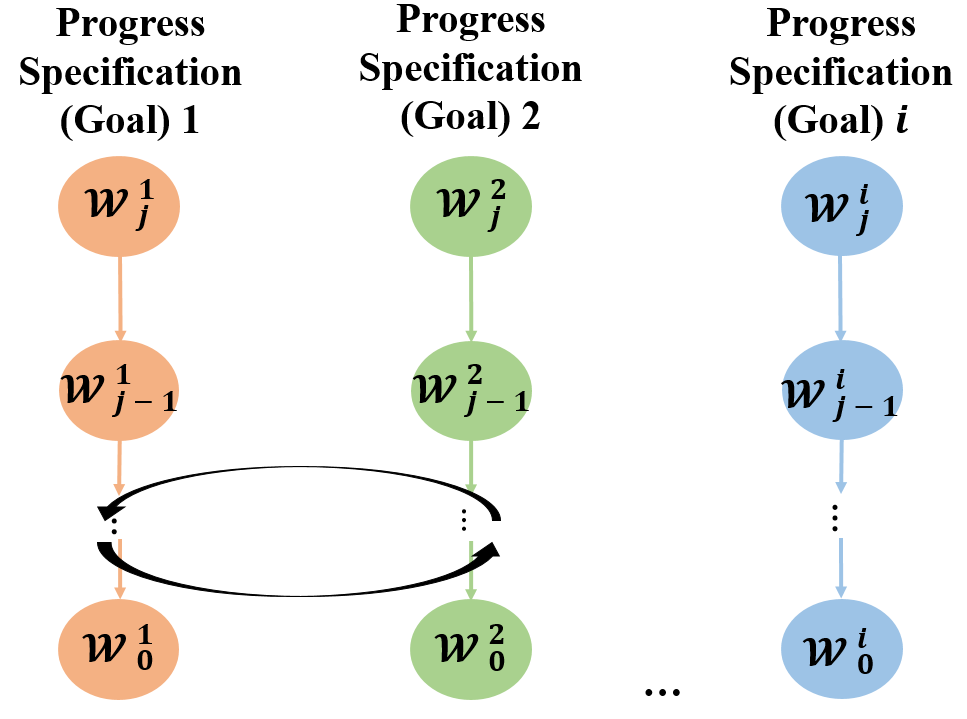
\includegraphics[width = 0.9 \linewidth]{AllocandGoals}
	\centering
	\caption{Diagram of allocation process rearranging the progress goal ordering (as depicted in Fig. \ref{RhFrame}) for a single UAV controller instance in real-time}
	\label{AllocandGoal}
	\vspace*{-3mm}
\end{figure}


As shown in Fig \ref{RHAlloc}, a common synthesized controller is created for each of the UAVs through the RH framework with the duties presented. Given any arbitrary initial condition, the controller aims to progress to each partitioned space, these goals represented within Fig. \ref{RHAlloc} by the ``nodes" protruding from each rectangle. The order that the controller meets these progress statements for a single UAV, shown previously through the ordering of $\mathscr{W}^i$ in Fig. \ref{RhFrame}, is not dictated by the synthesized controller as typically performed within the RH framework. Instead, the allocation process decides which progress specification any single UAV should pursue, represented within Fig. \ref{AllocandGoal} by the switching of the ``nodes'" order for any given moment in time. Hence, the allocation process prioritizes and assigns which goals a single controller should meet next in real-time. The combination of these two methods in the described manner works to highlight the strengths of each method. The synthesized controllers manage various system oriented aspects of the design and path planning while allocation governs the fleet behavior through assignments of goals for each controller.

Previously mentioned in \cite{c2}, a physical scenario was constructed that dealt solely with one UAV gathering water, moving to another location, and dumping said water on the destination. \cite{c2} demonstrates the existence of lower level controllers that could manage the individual actions necessary to achieve the high-level planner and controller this paper proposes (at least for a smaller scale UAV). So, as often expressed in other sources dealing with high-level synthesized controllers, we assume there exists low-level controllers to dictate the motion of individual agents in real-time.

One caveat with regards to the solution explored in this paper is the, perhaps obvious, alternative solution. Suppose the design was created through a more ``handcrafted" approach, one without the uses of formal methods for verification. Utilization of a path planning algorithm (such as any of the on-line algorithms discussed in \cite{c18}) for sending UAVs to any given destination (i.e. a fire or base) from any starting condition, could be combined with the described top-level allocation process that managed the destinations for all UAVs together. A huge benefit of such an approach is that the dedicated path-planning algorithm could handle a greater variety of dynamic environments than a synthesized controller. However, the described approach could easily be susceptible to programming errors due to the necessity of creating the conditions that dictate other task-oriented operations of the UAV (such as those involving control of the water level, knowing when to land under what conditions, etc.), precisely the issue that reactive synthesis aims to resolve. This paper's proposed solution method seeks to explore and expand the capabilities of reactive synthesis as a formal method within a more granular environment and complex task space.

\vspace*{-3mm}
\section{Implementation}

This section describes the construction and operation of the synthesized controllers and allocation algorithm used for the high-level controller. Additionally, the simulation used to test such cases is also outlined.

\vspace*{-3mm}
\subsection{Synthesis of Controllers in Receding Horizon framework}
For the common synthesized controller, environmental variables as perceived by a single UAV were created. These Boolean variables consist of: $StopSignal$, representing whether or not the UAV needs to stop due to periodic engine failures; $Fire$, representing the presence of fire directly beneath the UAV; and $DropWater$, representing allocation signaling a UAV to drop water on the assigned goal location. Hence, the environment $E = StopSignal \times Fire \times DropWater$. The system consists of $S$ as described in \textit{Section III}. Additional APs $GoalPos_i$ and $Base$ were created for when the UAV enters any specified goal location (indexed with $i \in I_g$) and the Base location, respectively.

The overall environment specifications for a single UAV are listed as follows: 
\begin{equation}
\varphi_{init}^{e} = \lnot StopSignal \land \lnot Fire,
\label{EnvInit}
\end{equation}
\begin{equation}
\varphi_{s}^{e} = \{\},
\label{EnvSafety}
\end{equation}
\begin{equation}
\begin{aligned}
\varphi_{p}^{e} = \always \eventually DropWater \land \always \eventually \lnot StopSignal \land \always \eventually \lnot Fire,
\end{aligned}
\label{envprog}
\end{equation}
Eq. (\ref{EnvInit}) formulates the idea that no UAV starts with engine failure or fire beneath it. (\ref{EnvSafety}) shows no guarantees on the environments behavior, and (\ref{envprog}) states that always eventually allocation instructs the UAV to drop water, the UAV will experience engine failure, and the UAV will not be over fire.

The overall system specifications for each UAV are listed:
\begin{equation}
\varphi_{init}^{s} = \Phi \land (w = 4).
\label{UAVinit}
\end{equation}
Eq. (\ref{UAVinit}) reflects that a UAV will start in the position and orientation states allowed by $\Phi$ (tautology that governs feasible states) and will start with the full water supply.
\begin{equation}
\begin{aligned}
\varphi_{s,1}^{s} = \always (StopSignal \land \lnot Fire \rightarrow sys\_actions = ``Stop"),
\end{aligned}
\label{UAVStop}
\end{equation}
Eq. (\ref{UAVStop}) states that a UAV experiencing the engine fail signal and is not over fire will stop in the current partition.
\begin{equation}
\begin{aligned}
\varphi_{s,2}^{s} = \always (\lnot ( StopSignal \land \lnot Fire ) \rightarrow \\ sys\_actions = ``Go"),
\end{aligned}
\label{UAVGo}
\end{equation}
Eq. (\ref{UAVGo}) indicates that in the negation of the previous condition, the UAV must transition to new partitions.
\begin{equation}
\begin{aligned}
\varphi_{s,3,i}^{s} = \always ((\lnot ( w = 0 ) \land DropWater \land \next GoalPos_i \land \lnot (\next Base)) \\ \rightarrow ((\next w) = (w - 1)),
\end{aligned}
\label{UAVWaterLevel}
\end{equation}
Eq. (\ref{UAVWaterLevel}), which exists for every goal AP, states that the next water level decrease by 1 if the water level isn't empty, the UAV is told to drop water into its goal, the UAV will transition into the goal next move, and the next move doesn't result in \textit{True} for $Base$.
\begin{equation}
\begin{aligned}
\varphi_{s,5,i}^{s} = \always ((( w = 0 ) \land DropWater \land \next GoalPos_i \land \lnot (\next Base)) \\ \rightarrow ((\next w) = w ),
\end{aligned}
\label{UAVWaterLevel3}
\end{equation}
Eq. (\ref{UAVWaterLevel3}) indicates that if the same conditions as (\ref{UAVWaterLevel}) hold except the water level is at empty, the water level must stay the same.
\begin{equation}
\begin{aligned}
\varphi_{s,4,i}^{s} = \always ((\lnot (DropWater \land \next GoalPos_i \land \next Base \rightarrow \\ ((\next w) = w),
\end{aligned}
\label{UAVWaterLevel2}
\end{equation}
Eq. (\ref{UAVWaterLevel2}) states that the water level will remain the same as before if the UAV is not told to drop water into its goal, is not transitioning into the goal next move, and/or is not transitioning to the base location.
\begin{equation}
\begin{aligned}
\varphi_{p,i}^{s} = \always \eventually DropWater \rightarrow GoalPos_i,
\end{aligned}
\label{UAVProg}
\end{equation}
Lastly, (\ref{UAVProg}) states that for every goal $i$, the UAV will transition into the goal location if the UAV is told to drop water.

% \begin{figure}
%	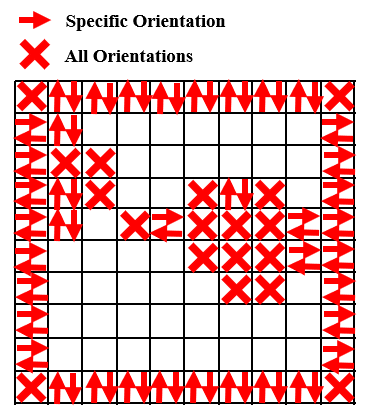
\includegraphics[width = 0.5 \linewidth]{Phi}
%	\centering
%	\caption{All positions and orientations not included in $\Phi$}
%	\label{Phi}
%\end{figure}

\begin{figure}
	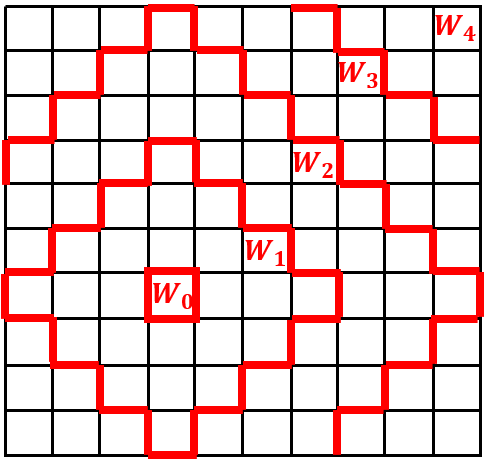
\includegraphics[width = 0.5 \linewidth]{WPartitionPic}
	\centering
	\caption{RH partitions for progress statement centered on position (4,4)}
	\label{WPart}
	\vspace*{-3mm}
\end{figure}


Given any excessively large values for $i \in I_g$, the total specification would yield a synthesized controller that would first, take an excessive amount of time to generate (longer than the 12 hours taken for an attempt with a 3.2 GHz processor), and second, create no practical performance with regards to extinguishing fires. From such, though, the RH framework is applied to the synthesized controller, as followed from \cite{c10}. For every progress specification, the partitioned grid is further segmented into subregions $\mathcal{W}_j^i$, an example of which is shown in Fig. \ref{WPart}. As displayed, the regions are ordered by $j$ based on their distance from the position that fulfills the particular progress statement (the $i$ index is not shown).

\begin{figure}
	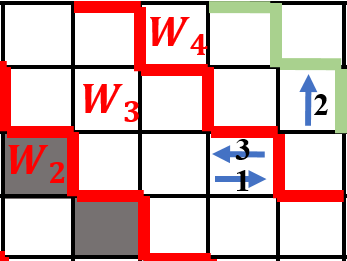
\includegraphics[scale=0.3]{ModifiedTran}
	\centering
	\caption{Limited (in red) and expanded (in green) transition space example for $\mathcal{W}_3$, with progress goals highlighted gray. Modified transition example shown by blue arrows.}
	\label{ModTran}
	\vspace*{-3mm}
\end{figure}


For each set of partitions $\mathcal{W}_j^i$, GR(1) specifications (of the form in (\ref{RH})) were constructed to enable correct transitions for the synthesized controllers. These specifications were differentiated between $j > 1$ and $j = 1$ through the progress statements and sets of initial conditions. For $j > 1$, the progress statements were constructed simply to force the UAV to transition into partitions contained within the next $\mathcal{W}$, an example of such shown in Fig. \ref{ModTran} through the highlighted partitions. For $j = 1$, the progress statements were constructed as discussed earlier with (\ref{UAVProg}).

\subsubsection{Receding Horizon Modification}

Also displayed in Fig. \ref{ModTran} is an example of the expanded transition spaces (cut out segments of $\mathcal{W}_4$) only used when initial conditions that do not provide feasible transitions to the next inner $\mathcal{W}$ arise. These situations typically occur around obstacles. Normally in an RH framework, infeasible initial conditions would be limited through the ordered sequence of progress goals. Due to the fact that any goal can proceed any other goal for this problem statement, though, all initial conditions for any $\mathcal{W}$ must be viable. The addition of these expanded transition spaces for the normally infeasible initial conditions provides a feasible transition path that the UAV moves into if needed. The planner that manages which synthesized controllers to use then switches to the one associated with set $\mathcal{W}_{j+1}$. Note that the synthesized controllers with these expanded transition spaces only exist for initial conditions that cannot transition to the next set $\mathcal{W}_{j-1}$. Unfortunately, the guarantee that the combined controller will always satisfy the specifications is lost anytime these synthesized controllers are used. From testing, though, we found that this issue only occasionally resulted in goal accessibility problems for UAVs assigned to fires directly on the other side of the larger obstacles. 

\vspace*{-4mm}
\subsection{Dynamic allocation}

In this paper, we propose an efficient method for managing the dynamic allocation of UAVs to fire locations that spread with time. The allocation process considers two paramaters, fire density and proximity of the UAVs to fire locations. Regions with higher fire densities correspond to areas with a higher number of fires concentrated in a region. To partition the map into regions according to their fire densities, the first step in our allocation process is to carry out the K-means $clustering$ $algorithm$ via the Matlab built-in function, $kmeans$. We set this function to use the Manhattan distance as the evaluation index of similarity in order to group fires with similar locations into the same cluster. The $kmeans$ function requires a desired number of clusters, $k$, as input. 

To find the optimal $k$, $k_{opt}$, the elbow method is used. [Similar work on utilizing the elbow method and other clustering techniques is shown in \cite{17}.] In the elbow method, the process iterates through the possible number of clusters, $k$, from 2 to some maximum number of clusters, $K_{max}$, and the sum of square error ($SEE$) for each $k$ is computed. Ideally, we are looking for a value of $k$ that results in clusters that have a low $SEE$. This would lead to fires with high location similarity being assigned to the same cluster. The optimal number of clusters is the value of $k$ at which the second derivative of the average of $SEE(k)$ is maximized. The idea is that the marginal drop in the average $SEE$ as $k$ increases will decrease dramatically for some value of $k$ before it reaches a plateau, hence the ``elbow criterion" The partition algorithm is summarized in Algorithm I.
\begin{algorithm}
	\caption{Partition algorithm}\label{alg:kMeans}
	\begin{algorithmic}[1]
		\Procedure{clustering}{$K_{max},fireLocs$}
		\State Set $k = 2$
		\While{$k < K_{max}$} 
		\State Compute clusters set $C = kmeans(fireLocs,k)$ 
		\State Compute mean sum of square error with k clusters, $SEE_{avg}(k)$
		\EndWhile
		\State Set optimal $k$, $k_{opt} = k$ that maximizes the second derivative of $SEE_{avg}(k)$
		\State Generate initial cluster centroid positions $C_{init}$
		\State Compute clusters set $C = kmeans(fireLocs,k_{opt},C_{init})$
		\State Assign $fireLocs$ to their corresponding cluster $c \in C$, 
		\State \textbf{return} $C$, fire location assignments
		\EndProcedure
	\end{algorithmic}
\end{algorithm}

Once the map is divided into clusters, the number of UAVs that will be allocated to each cluster is defined by (\ref{NAlloc}),
\begin{equation}
\label{NAlloc}
N_{alloc}(c) = \ceil[\big]{\rho_{c}/\rho_{tot}\times(N_{tot} - N_{free})},
\end{equation}
where $\rho_{c}$ is the cluster priority calculated as the sum of fire intensity values that belong to cluster $c$, $\rho_{tot}$ is the sum of intensity values of all fires. $N_{tot}$ is the total number of UAVs and $N_{free}$ is the number of UAVs that have not been assigned to a cluster. For each cluster $c$, we assign a subset of UAVs chosen from all available UAVs. This subset of size $N_{alloc}$ is comprised of those UAVs with locations closest to $c$. Once each cluster $c$ has an assigned subset of UAVs, the next step is to decide on which fire location in $c$ each UAV should go to. We have two modes in which UAVs can be assigned to fires, $Sync$ mode and $NonSync$ mode. 

In $Sync$  mode, for each cluster $c$, we pick the UAV in the subset of UAVs assigned to $c$ that is the closest to $c$ and determine the fire location with the minimum cost relative to this UAV. This cost is calculated as the weighted sum of the distance between the fire and the UAV, the fire intensity and its distance from the centroid of $c$, and the switching fires penalty for the UAV. The rest of the UAVs in the subset are assigned to the same fire. We refer to this cost fuction as $g$ as shown in (\ref{AllocEqn}).
\begin{equation}
\label{AllocEqn}
\begin{aligned}
\min_{f\in F} g(f,x) = d_{f}*\norm{x-f} + s_{f}*\norm{g-f} - \\ n_{f}*(f_{int} + \norm{c_{centroid}-f}),
\end{aligned}
\end{equation}
where $d_{f}$ (assigned as 0.3 in our simulation) is a coefficient between 0.0 and 1.0 and is used as an importance weight for the distance between UAV location $x$ and fire $f$ $\in$ $F$. $F$ represents the set of all fire locations in cluster $c$. The coefficient $n_{f}$ represents an importance weight for the fire intensity level, $f_{int}$, and the distance between the fire location and the centroid of cluster $c$. This coefficient is set as 1.0 - $d_{f}$. The first term in (\ref{AllocEqn}) seeks to drive UAVs towards their closest fires while the second term seeks to prioritize outer fires with higher intensities. Finally, coefficient $s_{f}$ corresponds to the switching penalty for when an already assigned fire changes to a different fire (assigned as 10 in our simulation). This prevents UAVs from going to different fires if they have not yet reached their previously assigned fire. If the UAV reaches its assigned fire, then the minimization is done over all other fires.  

In $NonSync$ mode, for each cluster $c$, we loop through each UAV from the subset of UAVs assigned to $c$ and proceed with the minimization, but only one UAV is assigned to a single fire. The fire is chosen from the set of unassigned fires for each UAV according to (\ref{AllocEqn}). Each time a fire is assigned, it is removed from the set $F$. 

\vspace*{-4mm}
\subsection{Simulation}

To implement the solution and test its ability to meet the problem scenario, the synthesized controllers and allocation algorithm were constructed in MATLAB with a step-based simulation in mind, i.e. the simulation's main loop updated upon each move performed by the synthesized controllers. The time scale of the loop was adjusted to match that of a UAV's transition from one partition to the next, since most controller moves related to time revolved around such. From this, longer time-based actions, such as the fires' described spreading behaviors and the UAVs' wait times, were only updated when the amount of loops corresponding to the desired amount of time passed.

\begin{figure}
	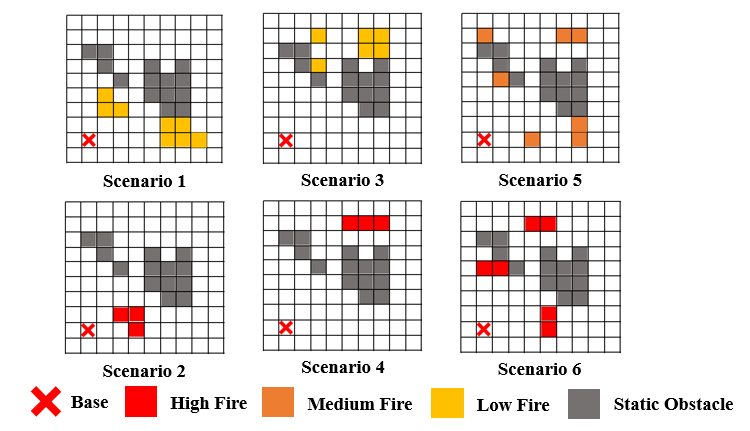
\includegraphics[width = 1 \linewidth]{scenariosFire}
	\centering
	\caption{Fire scenario visualizations, initial conditions}
	\label{scenarioFire}
	\vspace*{-3mm}
\end{figure}

Furthermore, various fire scenarios' initial conditions were constructed for the purposes of testing the controllers. These fire scenarios were aimed at testing the capabilities of the UAVs to extinguish all fires without the fuel decreasing below the minimum amount, with no exact focus on performance. The simulation cycled through iterations on each scenario, increasing the number of UAVs until the goal was met. Additionally, the scenarios aimed to capture a wide range of initial conditions and assess the differences between the allocation's \textit{Sync} and \textit{NonSync} modes. The exact initial fire placements are depicted in Fig. \ref{scenarioFire}. For all scenarios, the UAVs started at the base location.

\vspace*{-3mm}
\section{Results}

TuLiP \cite{c12} was utilized to realize and synthesize the controllers associated with each region $\mathcal{W}_j^i$. On an Intel i5-6500 CPU @ 3.20 GHz processor, this total process, approximately 250 regions $\mathcal{W}$, took on the order of 8 hours. In addition to the large amount of time to synthesize all of the individual controllers, numerous memory issues came up throughout the process, even with a system limit of 16 GB of RAM. The total size of the synthesized controllers was approximately 2 GB.

For each scenario tested, simulations where conducted 100 times to assess the fleet of UAVs' ability to meet the fire elimination and fuel sustainment goals described previously, provided each UAV experiences a 1\% chance of engine failure for every transition time (3 seconds in all scenarios). The minimum fuel amount was chosen as 84, about one fourth the starting fuel amount. The results were compiled into Table \ref{table_23}. Additionally, an example time lapse for Scenario 1 is presented in Fig. \ref{ResultsShow}, showcasing how the fire grew in response to a varying number of UAVs.

\begin{table}[H]
	\caption{Simulation results}
	\label{table_23}
	\scalebox{0.8}{
		\begin{tabular}{|c||c||c||c||c||c||c|}
			\hline
			\multicolumn{1}{|p{1.75cm}|}{\centering Scenario \\ number \\ (S - \textit{Sync}, \\ NS - \textit{NonSync})} & \multicolumn{2}{|p{2.5cm}|}{\centering Mean minimum \\ number of UAVs \\ required} & \multicolumn{2}{|p{2.5cm}|}{\centering Mean simulated \\ real-time (s) for \\ completion} & \multicolumn{2}{|p{2.5cm}|}{\centering Mean fuel \\ remaining} \\ 
			\hline
			\multicolumn{1}{|p{1.75cm}|}{\centering } & \multicolumn{1}{|p{1cm}|}{\centering S} & \multicolumn{1}{|p{1cm}|}{\centering NS} & \multicolumn{1}{|p{1cm}|}{\centering S} & \multicolumn{1}{|p{1cm}|}{\centering NS} & \multicolumn{1}{|p{1cm}|}{\centering S} & \multicolumn{1}{|p{1cm}|}{\centering NS} \\ 
			\hline
			1 & 2.95 & 2.96 & 3871.2 & 4344.8 & 274.6 & 273.3 \\ 
			\hline
			2 & 2.04 & 2.10 & 1910.6 & 1518.0 & 291.1 & 293.6 \\
			\hline
			3 & 2.04 & 2.08 & 11932.7 & 11170.0 & 156.3 & 169.0 \\
			\hline
			4 & 2.31 & 2.30 & 10224.8 & 10221.4 & 166.5 & 165.3 \\
			\hline
			5 & 4.00 & 4.05 & 8641.8 & 8431.2 & 200.8 & 200.0 \\
			\hline
			6 & 4.72 & 4.68 & 7500.1 & 7463.0 & 120.4 & 122.1 \\
			\hline
		\end{tabular}
	}
\vspace*{-3mm}
\end{table}

\begin{figure}
	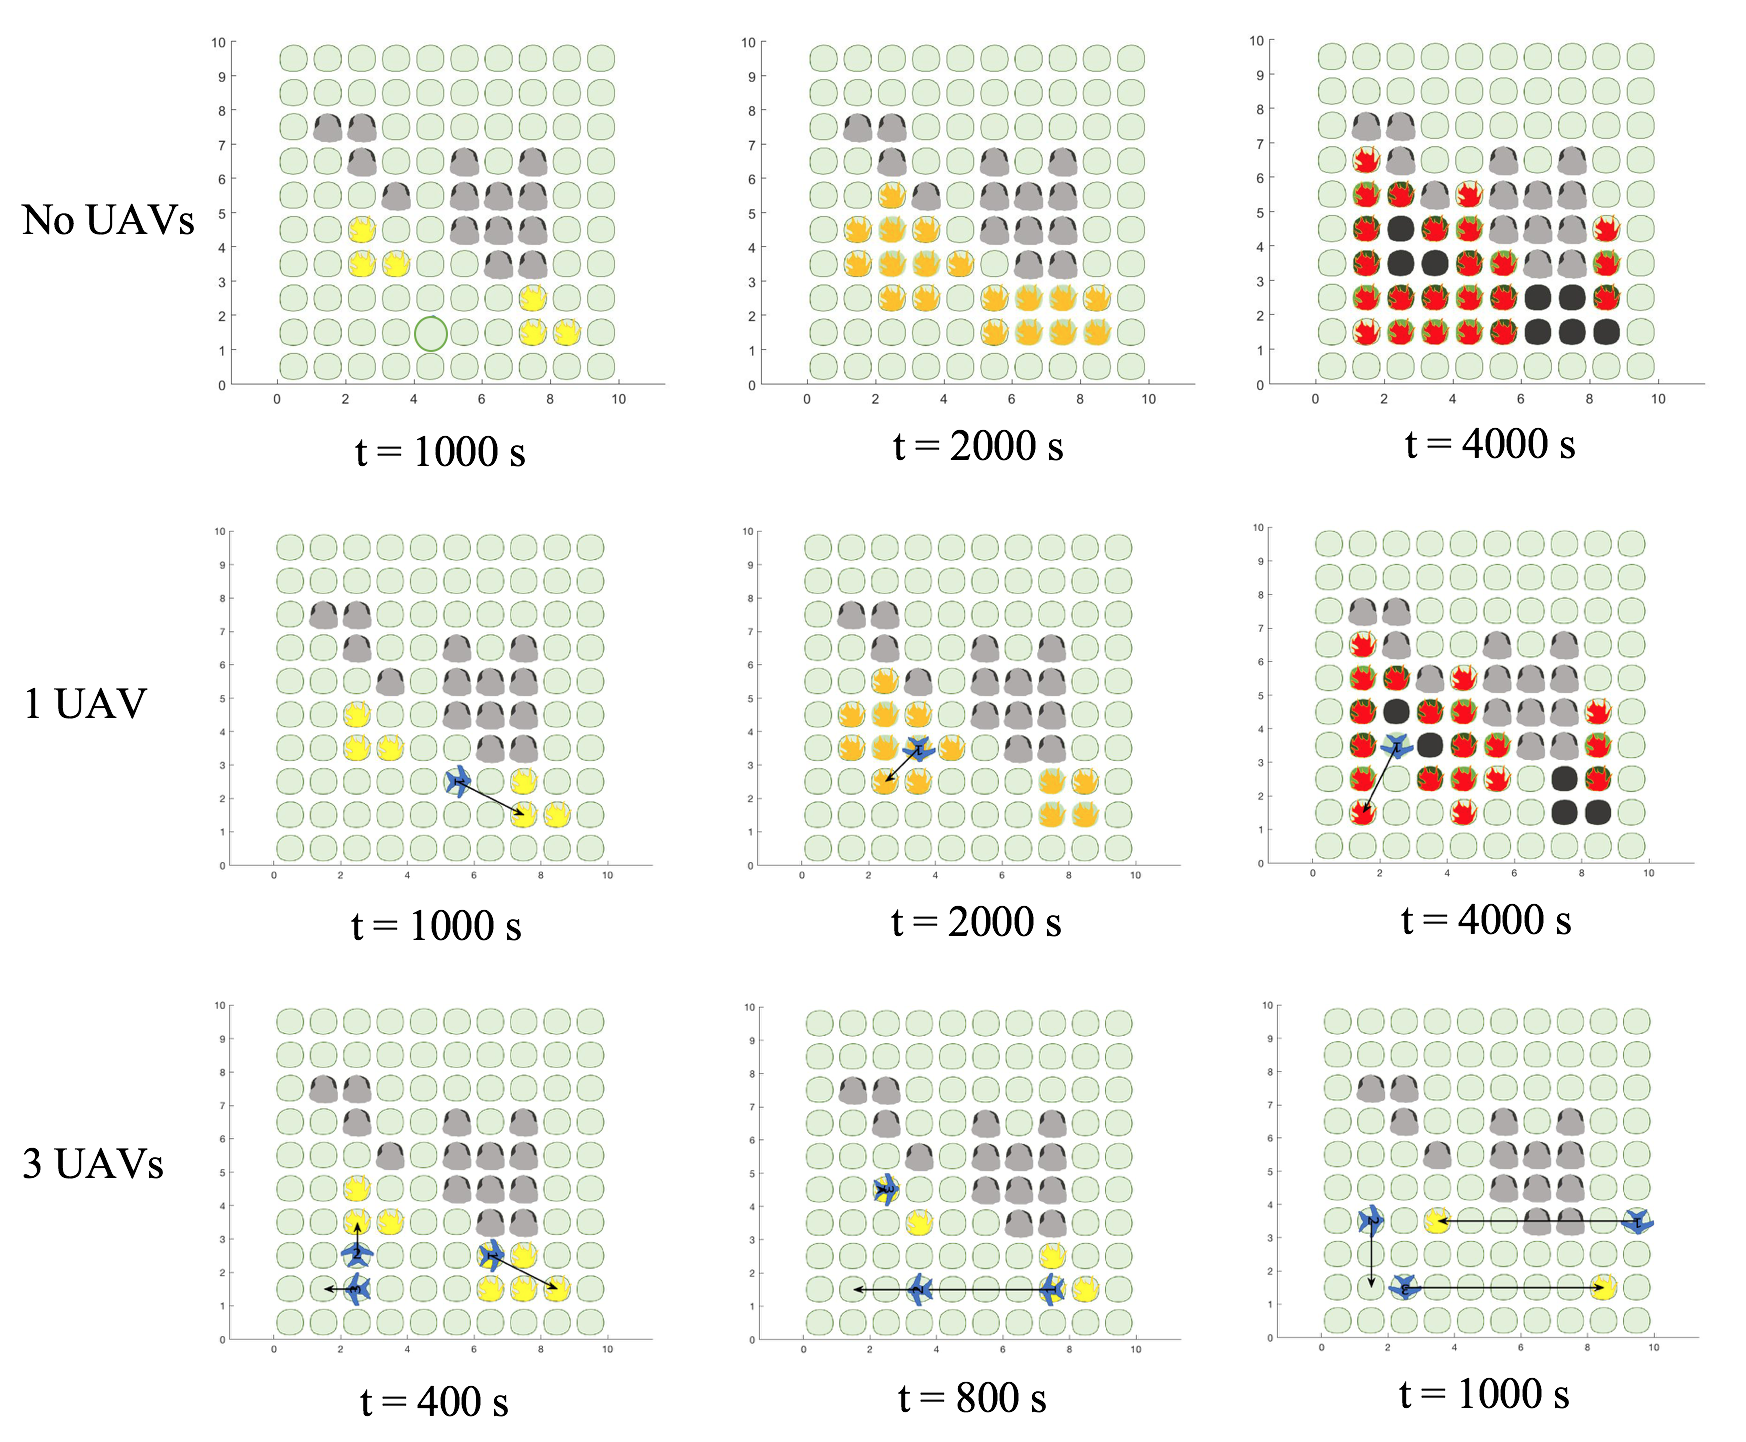
\includegraphics[width = 1 \linewidth]{ResultsShow}
	\centering
	\caption{Example of scenario 1 results for no UAVs, 1 UAV, and 3 UAVs, with success shown in the last case}
	\label{ResultsShow}
	\vspace*{-2mm}
\end{figure}

As shown by the mean values in Table \ref{table_23}, each case required no more than 5 UAVs on average to meet the prescribed objectives. Marginal differences existed between the \textit{Sync} and \textit{NonSync} modes for each scenario, with the largest differences displayed between the time for completion and the remaining fuel. It would appear that the number of UAVs used by the allocation algorithm had a greater impact on the results than the mode used. This outcome is highlighted by the marginal differences between the modes for each scenario compared to the differences between each scenario in general. Otherwise, in general, the longer the UAVs spent fighting the fires and the more intense the fires were resulted in greater fuel loss, an expected result.  

\vspace*{-3mm}
\section{Conclusion and Future Work}

In this paper, we constructed a high-level planner and controller to control a fleet of UAVs for various fire fighting scenarios. We simulated this method's ability to meet the objectives of eliminating all fires without losing more than a set amount of forestry through 6 varied scenarios, demonstrating success with no more than 5 UAVs needed on average.

Expanding upon the receding horizon framework for reactive synthesis allowed us to expand the scope of this problem while integrating the method with dynamic allocation for assigning UAVs. Even with such an approach, numerous issues arose throughout the process that help highlight key difficulties moving forward when using reactive synthesis in the control of UAVs. First, applying the $\mathscr{W}$ regions based primarily on position and ignoring orientations yields regions that prohibit specific initial conditions, especially with larger scale obstacles within the region. Our method of modified transition spaces circumvented the issues of synthesizing a controller at the loss of our guarantees for meeting the top level specification when such spaces are used. Second, the RH framework, when considering all initial conditions, still yields an excessively large controller (about 2 GB) after 8 hours of runtime. Lastly, a simplified transition system was utilized which limited the total orientation space and interpreted UAV movement in only 2 dimensions, still far more restrictive than UAV movement in reality. Each of these points combine to exemplify the need for smarter partitioning of possible transitions a UAV can take in 3D space (easily dependent on at least 3 full degrees of freedom), should reactive synthesize be used for UAV control.

For improvements on this problem as it was explored, further evaluation of the effectiveness of our solution needs to be assessed with regards to more scenarios. Furthermore, performance metrics with regards to time should be built into the specifications to ensure timely reactions to the environment, improving efficiency at fighting the fires. Lastly, a greater detail simulation, one that models the reactions and behaviors of the fire and UAVs in real-time (instead of move-based increments), would aid in better assessment of our solution.

\section{RH Proof}

\begin{definition}
	Left-total is defined for a set of states $s \in S$ and transitions $s \to s' \in R \subseteq S \times S$ as $\forall s \in S$ $\exists s' \in S$ such that $s \to s' \in R$
\end{definition}

\begin{definition}
	Right-total is defined for a set of states $s \in S$ and transitions $s \to s' \in R \subseteq S \times S$ as $\forall s' \in S$ $\exists s \in S$ such that $s \to s' \in R$
\end{definition}

\begin{definition}
	\label{definition3}
	Path-connectedness is used to refer to a state set and transition relation that is both left-total and right-total.
\end{definition}

\begin{definition}
	The state set is defined as $S = s_p \times s_o \times w$, where $s_p = \{1, 2, ...10\} \times \{1, 2, ...10\}$, $s_o = \{1, 2, 3, 4\}$, and $w = \{0, 1, 2, 3, 4\}$
\end{definition}

\begin{definition}
	For all $s_{i,p} \in s_p$, $g_i = \{s \in S$ $|$ $s_{i,p} \in s\}$. $g_{i,p}$ refers to the set $s_{i,p}$ that it was defined for.
\end{definition}

\begin{definition}
	\label{definition6}
	Horizons are defined as $\mathcal{W}^i_j = \{s \in S$ $|$ $|a[1]| + |a[2]|$ $ < 3*j$ and $s \not \in \mathcal{W}^i_{j-1},$ where $a = s_{i,p} - g_{i,p}$ and $j > 0\}$.
\end{definition}

\begin{definition}
	\label{definition7}
	The transition relation for the state set $S$ is defined as $T = \{s \to s' \in R \subseteq S \times S\}$, where elements $s \to s' \in R$ are defined for each of the following $s'$ definitions per $s \in S$. Note $s' \in S$ must be fulfilled. 
	
	If $s_o \in s = 1$, $s' = \{s_{i,p} + \{0,1\},1\}$, $s' = \{s_{i,p} + \{1,1\},2\}$, and $s' = \{s_{i,p} + \{-1,1\},4\}$. 
	
	If $s_o \in s = 2$, $s' = \{s_{i,p} + \{1,0\},2\}$, $s' = \{s_{i,p} + \{1,1\},1\}$, and $s' = \{s_{i,p} + \{1,-1\},3\}$. 
	
	If $s_o \in s = 3$, $s' = \{s_{i,p} + \{0,-1\},3\}$, $s' = \{s_{i,p} + \{1,-1\},2\}$, and $s' = \{s_{i,p} + \{-1,-1\},4\}$. 
	
	If $s_o \in s = 4$, $s' = \{s_{i,p} + \{-1,0\},4\}$, $s' = \{s_{i,p} + \{-1,-1\},3\}$, and $s' = \{s_{i,p} + \{-1,1\},1\}$.
\end{definition}

Assuming that the overall specification is synthesizable for the system description given no horizons and under any allowable initial condition, a horizon-based synthesized solution must also exist \textbf{(Do we need to restate RH framework conditions and outcomes to make this last statement apparent?)}. Given the receding horizon template pictured in Fig. \ref{WPart} and formally described in Definition \ref{definition6}, guarantees regarding the satisfaction of our overall specification through the RH framework can be provided under modified horizon definitions. The proof of such is provided using the following assumptions.

First, we only consider a subset of the total state definition that includes only location and orientation. This is directly allowed for all horizons since specifications regarding the water levels require the position and orientation states to reach desired goal locations $g_{i,p}$ (including the base of operations). This subset is defined as $S_{sub} = s_p \times s_o$. We assume that a further subset of $S_{sub}$ exists (coined $S_{s}$) such that, when combined with the transition relation defined by Definition \ref{definition7} having $S$ replaced by $S_s$, the total state set and transition relation holds path-connectedness as defined by Definition \ref{definition3}.

Our proof follows from the above assumptions. Given the description of the receding horizons $\mathcal{W}^i_j$ for any individual goal $g_i$, where $\mathcal{W}^i_0 = g_i$, path-connectedness implies that for any state sequence $\pi$ that starts and leads from $s \in \mathcal{W}^i_j$ to a state $s_f \in g_i$, said sequence $\pi$ must contain at least one $s \in \mathcal{W}^i_k$ for all $0 < k \le j$. Under the refined definition of $S_{s}$, all available $\pi$ sequences for some $s \in \mathcal{W}^i_j$ may also need to include $s \in \mathcal{W}^i_r$ for some $r > j$. The possibility of such a sequence that includes paths with $s \in \mathcal{W}^i_{r > j}$ immediately violates the conditions for the receding horizon specification $\Psi_{j}^{i}$ (defined by Eq. \ref{RH}). To revert such, a modification to the horizons is made during synthesis in order to maintain the condition that a path $\pi$ does not contain any $s \in \mathcal{W}^i_{r > j}$. This process is displayed in Algorithm \ref{alg:Wgen}.

\begin{algorithm}
	\caption{$\mathcal{W}^i_j$ Modification during Synthesis}\label{alg:Wgen}
	\begin{algorithmic}[1]
		\Procedure{Synthesis$\_$Goal}{$i$}\Comment{Synthesis controllers from all initial conditions for the $i$th goal location}
		\For{$0 \le j \le N$}
		\For{$s \in \mathcal{W}_j^i$}
		\State Synthesize controller given $g_i$ and current $s$
		\If{Controller == None}
		\State Remove $s$ from $\mathcal{W}_j^i$
		\State Add $s$ to $\mathcal{W}_{j+1}^i$
		\EndIf
		\EndFor
		\EndFor
		\EndProcedure
	\end{algorithmic}
\end{algorithm}			

As controllers are synthesized around each goal and for each initial condition within each set $\mathcal{W}^i_j$, starting with $j = 0$ and incrementing, realizability failures are direct results of the lack of a system path to the horizon $\mathcal{W}^i_{j-1}$ that remains only in $\mathcal{W}^i_{j}$ under the assumed environment conditions. This is a result of the failure to satisfy $\Psi_{j}^{i}$. \textbf{(Does this statement need further proof?)}. Because a path that fulfills the global specification must exist on the global scale and none of the sets $\mathcal{W}^i_j$ overlap per index $i$, \textbf{(Does this need further proof, or is it implied enough from earlier?)}, the path must enter into $\mathcal{W}^i_{j+1}$ due to the path connectedness property stated before. All intermediate states between the initial condition and horizon $\mathcal{W}^i_{j+1}$ are also moved to the next horizon since each state is tested as an initial condition in Algorithm \ref{alg:Wgen}, and these states cannot serve as viable initial conditions themselves. Therefore, the revised $\mathcal{W}^i_{j+1}$ contains the original set $\mathcal{W}^i_{j+1}$ plus all states from $\mathcal{W}^i_{j}$ that could not serve as initial conditions to reach the horizon/goal of $\mathcal{W}^i_{j-1}$. This statement serves as a recursive assignment for each horizon $j$, shifting states back horizons until a new horizon set for a goal is defined such that each $s \in \mathcal{W}^i_{j}$ starts a path $\pi$ contained solely in $\mathcal{W}^i_{j}$ that reaches $\mathcal{W}^i_{j-1}$. Because of this, $\Psi_{j}^{i}$ is realizable for all goals, all horizons, and all initial conditions, fulfilling the guarantees provided by the RH framework used. (\textbf{Don't think I need next sentence...})No new horizons are created at the domain edge since a viable controller must exist on the global scale (\textbf{Is this directly implied though or does it need further proof...?}).

The benefit of this approach is that the viability test for an initial condition is made during synthesis and construction of controllers, saving on computation time since the horizons aren't evaluated and modified before synthesis. Hence the original horizon definition serves as a starting point that may or may not be preserved for each goal and is only modified when necessary.


\vspace*{-3mm}
\begin{thebibliography}{1}
\bibitem{c0}	
D. Thomas, D. Butry, S. Gilbert, D. Webb, and J. Fung, ``The costs and losses of wildfires: a literature survey," \textit{Special Publication (NIST SP)}, Nov. 2017. 
\bibitem{c1}
D. Werner, ``Fire Drones," \textit{Aerospace America}, pp. 28–31, 2015. 
\bibitem{c10}
T. Wongpiromsarn, U. Topcu and R. M. Murray, ``Receding Horizon Temporal Logic Planning," \textit{IEEE Transactions on Automatic Control}, vol. 57, no. 11, pp. 2817-2830, Nov. 2012.	
\bibitem{c2}
H. Qin et al., ``Design and implementation of an unmanned aerial vehicle for autonomous firefighting missions," \textit{2016 12th IEEE International Conference on Control and Automation (ICCA)}, Kathmandu, pp. 62-67, 2016.
\bibitem{c3}
B. Johnson, F. Havlak, H. Kress-Gazit, and M. Campbell, ``Experimental Evaluation and Formal Analysis of High-Level Tasks with Dynamic Obstacle Anticipation on a Full-Sized Autonomous Vehicle," \textit{Journal of Field Robotics}, 2017.
\bibitem{c4}
K. W. Wong and H. Kress-Gazit, ``Need-based coordination for decentralized high-level robot control," \textit{2016 IEEE/RSJ International Conference on Intelligent Robots and Systems (IROS)}, Daejeon, pp. 2209-2216, 2016.
\bibitem{c5}
J. Alonso-Mora, J. A. DeCastro, V. Raman, D. Rus, and H. Kress-Gazit, ``Reactive mission and motion planning with deadlock resolution avoiding dynamic obstacles," \textit{Autonomous Robots}, 2017.
\bibitem{c14}
Z. Liang, X. Yang and Y. Deng, ``A partitioning-based task allocation strategy for Police Multi-Agents," \textit{ The 26th Chinese Control and Decision Conference (2014 CCDC)}, Changsha, pp. 2124-2128, 2014.
\bibitem{c15}
B. Mirzapour and H. S. Aghdasi, ``Modified multi-objective hybrid DE and PSO algorithms for resource allocation in forest fires," \textit{2017 7th International Conference on Computer and Knowledge Engineering (ICCKE)}, Mashhad, pp. 187-192, 2017.
\bibitem{16}
P. Fiorucci, F. Gaetani, R. Minciardi, R. Sacil and E. Trasforini, ``Dynamic resource allocation for forest fire risk management," \textit{Proceedings. 15th International Workshop on Database and Expert Systems Applications, 2004}, pp. 603-607, 2004.
\bibitem{c6}
J. Tumova and D. V. Dimarogonas, ``Multi-agent planning under local LTL specifications and event-based synchronization," \textit{Automatica}, vol. 70, pp. 239-��248, 2016.
\bibitem{c7}
N. Piterman, A. Pnueli, and Y. Saar, ``Synthesis of reactive (1) designs, in Verification, Model Checking, and Abstract Interpretation." Springer, pp. 364-380, 2006.
\bibitem{c8}
A. Ulusoy and C. Belta, ``Receding horizon temporal logic control in dynamic environments," \textit{The International Journal of Robotics Research}, vol. 33 , no. 12, pp. 1593-��1607, Jul. 2014.
\bibitem{c9}
X. C. Ding, M. Lazar and C. Belta, ``Receding horizon temporal logic control for finite deterministic systems," \textit{2012 American Control Conference (ACC)}, Montreal, QC, pp. 715-720, 2012.
\bibitem{c11}
M. P. Plucinski, A. L. Sullivan, and R. J. Hurley, ``A methodology for comparing the relative effectiveness of suppressant enhancers designed for the direct attack of wildfires," \textit{Fire Safety Journal}, vol. 87, pp. 71-��79, 2017.
\bibitem{c18}
Liang Yang, Juntong Qi, J. Xiao and Xia Yong, ``A literature review of UAV 3D path planning," \textit{Proceeding of the 11th World Congress on Intelligent Control and Automation}, Shenyang, pp. 2376-2381, 2014.
\bibitem{17}
P. Bholowalia and A. Kumar, ``EBK-Means: A Clustering Technique based on Elbow Method and K-Means in WSN," \textit{International Journal of Computer Applications}, vol. 15, no. 9, pp. 17-24, 2014.
\bibitem{c12}
T. Wongpiromsarn, U. Topcu, N. Ozay, H. Xu, and R. M. Murray, ``TuLip: A software toolbox for receding horizon temporal logic planning," \textit{Proc. Int. Conf. Hybrid Syst.: Computat. Control}, pp. 313-��314, 2011.



\end{thebibliography}
% biography section
% 
% If you have an EPS/PDF photo (graphicx package needed) extra braces are
% needed around the contents of the optional argument to biography to prevent
% the LaTeX parser from getting confused when it sees the complicated
% \includegraphics command within an optional argument. (You could create
% your own custom macro containing the \includegraphics command to make things
% simpler here.)
%\begin{IEEEbiography}[{\includegraphics[width=1in,height=1.25in,clip,keepaspectratio]{mshell}}]{Michael Shell}
% or if you just want to reserve a space for a photo:
%\begin{IEEEbiographynophoto}{Estefany Carrillo}
%is an graduate student at the University of Maryland, College Park, in the %Department of Electrical Engineering. She received her BS degree and M.S. in %electrical engineering from University of Maryland in 2012 and 2017, respectively.  
%\end{IEEEbiographynophoto}
% if you will not have a photo at all:

% that's all folks
\end{document}


